\documentclass[margin=5pt,
  convert,
  convert={
    outext=.png,
    command=\unexpanded{
      pdftocairo -r 600 -png \infile % 将生成的pdf文件转换为png图像
    }
  }
]{standalone}

% 支持中文
\usepackage{ctex}
% 流程图绘制宏包
\usepackage{tikz}
\usetikzlibrary{arrows.meta}

% 设置流程图绘制参数

\begin{document}

\newpage

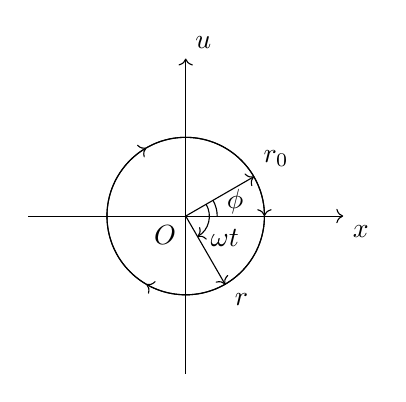
\begin{tikzpicture}
    \draw[->] (-2,0) -- (2,0); 
    \draw[->] (0,-2) -- (0,2);
    \draw[->] (0,0) -- (30:1);
    \draw[->] (0,0) -- (-60:1);
    \node[below right] (B) at (2,0) {$x$};
    \node[below right] (E) at (-15:0.2) {$\omega t$};
    \node[above right] (C) at (0,2) {$u$};
    \node[below left] (O) at (0,0) {$O$};
    \node[above right] (D) at (30:1) {$r_0$};
    \node[above right] (G) at (0.4,-0.1) {$\phi$};
    \node[below right] (F) at (-60:1) {$r$};
    \draw (0,0) circle (1cm);
    \draw[->] (240:1) arc [start angle=240, end angle=120, radius=1cm];
    \draw[->] (1,0) arc [start angle=360, end angle=240, radius=1cm];
    \draw[->] (120:1) arc [start angle=120, end angle=0, radius=1cm];
    \draw[->] (30:0.3) arc [start angle=30, end angle=-60, radius=0.3cm];
    \draw (0.4,0) arc [start angle=0, end angle=30, radius=0.4cm];
\end{tikzpicture}

\newpage

\begin{tikzpicture}
  \draw[->] (-2,1) -- (2,1); 
  \draw[->] (-2,0) -- (3,0); 
  \draw[->] (-2,-1) -- (2,-1); 
  \draw[->] (0,-2) -- (0,2);
  \node[above left] (A) at (2,1) {$E$};
  \node[below right] (B) at (3,0) {$x$};
  \node[above right] (C) at (0,2) {$y$};
  \node[below right] (O) at (0,0) {$O$};
  \fill (-1,0.5) circle (2pt);
  \fill (-1,-0.5) circle (2pt);
  \fill (1,0.5) circle (2pt);
  \fill (1,-0.5) circle (2pt);
  \node[above left] (A) at (-1,0.5) {$B$};
  \draw[->] (0,0) -- (30:1);
  \node[above left] (O) at (30:1) {$v_0$};
  \node[below right] (O) at (0.33,0.44) {$\theta_0$};
  \draw (0:0.3) arc [start angle=0, end angle=30, radius=0.3cm];
\end{tikzpicture}

\newpage

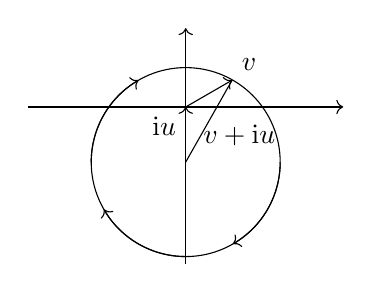
\begin{tikzpicture}
  \draw[->] (-2,0) -- (2,0); 
  \draw[->] (0,-2) -- (0,1);
  \draw[->] (0,0) -- (30:0.68);
  \draw[->] (0,-0.7) -- (0,0);
  \draw (0,-0.7) circle (1.2cm);
  \draw (0,-0.7) -- (30:0.68);
  \node[below left] (O) at (0,0) {$\mathrm{i} u$};
  \node[above right] (A) at (30:0.68) {$v$};
  \node[below right] (B) at (0.1,-0.1) {$v+\mathrm{i} u$};
  \draw[->] (1.2,-0.7) arc [start angle=0, end angle=-60, radius=1.2cm];
  \draw[->] (0,-1.9) arc [start angle=-90, end angle=-150, radius=1.2cm];
  \draw[->] (-1.2,-0.7) arc [start angle=180, end angle=120, radius=1.2cm];
\end{tikzpicture}

\newpage

\begin{tikzpicture}
  \draw[->] (0,-1.5) -- (0,2.3);
  \draw[->] (8,0) -- (-1.5,0); 
  \draw (0,1) circle (1cm);
  \node[below right] (B) at (-2,0) {$y$};
  \node[above right] (C) at (0,2) {$x$};
  \draw[domain=0:8.4,smooth] plot({\x-sin(\x r)},{1-cos(\x r)});
  \draw (4,1) circle (1cm);
  \draw[->] (0,1) -- (0,0);
  \draw[->] (4,1) -- (4.7,1.7);
  \draw[->] (4,1) -- (4.7,1.7);
\end{tikzpicture}

\newpage

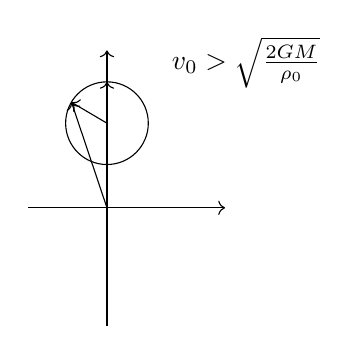
\begin{tikzpicture}
  \draw[->] (-1,0) -- (1.5,0); 
  \draw[->] (0,-1.5) -- (0,2);
  \draw[->] (0,0) -- (0,1.6);
  \draw[->] (0,1.075) -- (-0.45,1.34);
  \draw[->] (0,0) -- (-0.45,1.34);
  \draw (0,1.075) circle (0.525cm);
  \node[above right] (C) at (0.7,1.4) {$v_0>\sqrt{\frac{2GM}{\rho_0}}$};
\end{tikzpicture},
\begin{tikzpicture}
  \draw[->] (-1.5,0) -- (1.5,0); 
  \draw[->] (0,-1.5) -- (0,2);
  \draw[->] (0,0) -- (0,1.4);
  \draw[->] (0,0.7) -- (-0.6,1.05);
  \draw[->] (0,0) -- (-0.6,1.05);
  \draw (0,0.7) circle (0.7cm);
  \node[above right] (C) at (0.7,1.4) {$v_0=\sqrt{\frac{2GM}{\rho_0}}$};
\end{tikzpicture},
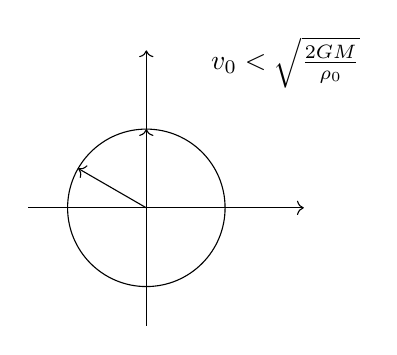
\begin{tikzpicture}
  \draw[->] (-1.5,0) -- (2,0); 
  \draw[->] (0,-1.5) -- (0,2);
  \draw[->] (0,0) -- (0,1);
  \draw[->] (0,0) -- (150:1);
  \draw (0,0) circle (1cm);
  \node[above right] (C) at (0.7,1.4) {$v_0<\sqrt{\frac{2GM}{\rho_0}}$};
\end{tikzpicture} 

\begin{tikzpicture}
  \draw[->] (0,0)--(7,0);
  \node[below left] (C) at (0,0) {$O$};
  \node[below left] (C) at (2.3,0) {$\frac12$};
  \node[below right] (C) at (2,2) {$1$};
  \node[below right] (C) at (5,0) {$B$};
  \node[below left] (C) at (2,1.2) {$A$};
  \draw (0,0) -- (0,2);
  \draw (2,0) -- (2,2);
  \draw (0,2) -- (5,0);
\end{tikzpicture} 
\end{document}